\begin{figure}[htbp]
\centering
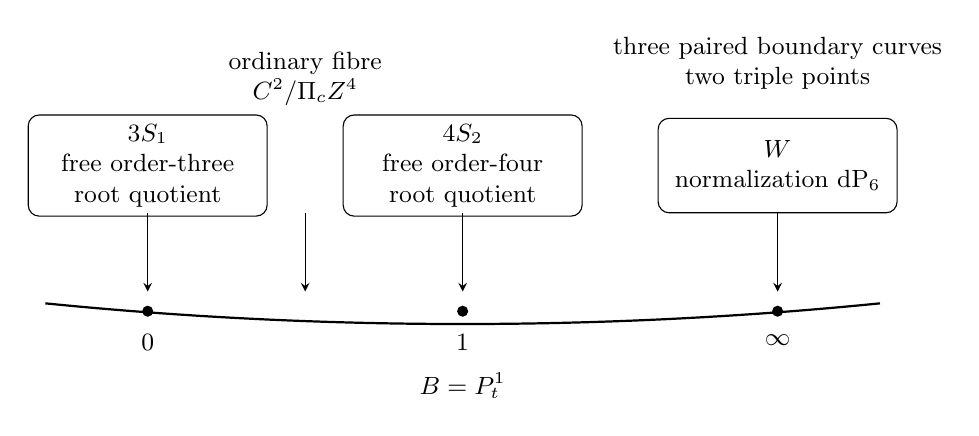
\begin{tikzpicture}[x=1cm,y=1cm,>=stealth,font=\small]
\draw[thick] (-5.3,0) .. controls (-1.8,-.35) and (1.8,-.35) .. (5.3,0);
\node at (0,-1.05) {$B=\mathbb P^1_t$};
\foreach \x/\lab in {-4/0,0/1,4/\infty}{
 \fill (\x,-.1) circle (2pt);
 \node[below=5pt] at (\x,-.1) {$\lab$};
 \draw[->] (\x,1.15)--(\x,.15);
}
\node[draw,rounded corners,align=center,text width=2.8cm,minimum height=1.2cm] at (-4,1.75)
 {$3S_1$\\free order-three\\root quotient};
\node[draw,rounded corners,align=center,text width=2.8cm,minimum height=1.2cm] at (0,1.75)
 {$4S_2$\\free order-four\\root quotient};
\node[draw,rounded corners,align=center,text width=2.8cm,minimum height=1.2cm] at (4,1.75)
 {$W$\\normalization $\mathrm{dP}_6$};
\draw[->] (-2,1.15)--(-2,.15);
\node[align=center] at (-2,2.85) {ordinary fibre\\$\mathbb C^2/\Pi_c\mathbb Z^4$};
\node[align=center] at (4,3.05) {three paired boundary curves\\two triple points};
\end{tikzpicture}
\caption{The fixed $(3,4,\infty)$ base data. The arrows denote the
restriction of $f$ to each indicated fibre, with its scheme
multiplicity retained. The ordinary period quotient, finite affine
quotients and the paired hexagon are the three actual local models
in the common conventions; their overlap maps are fixed there.}
\label{fig:I:orbifold}
\end{figure}

\begin{figure}[htbp]
\centering
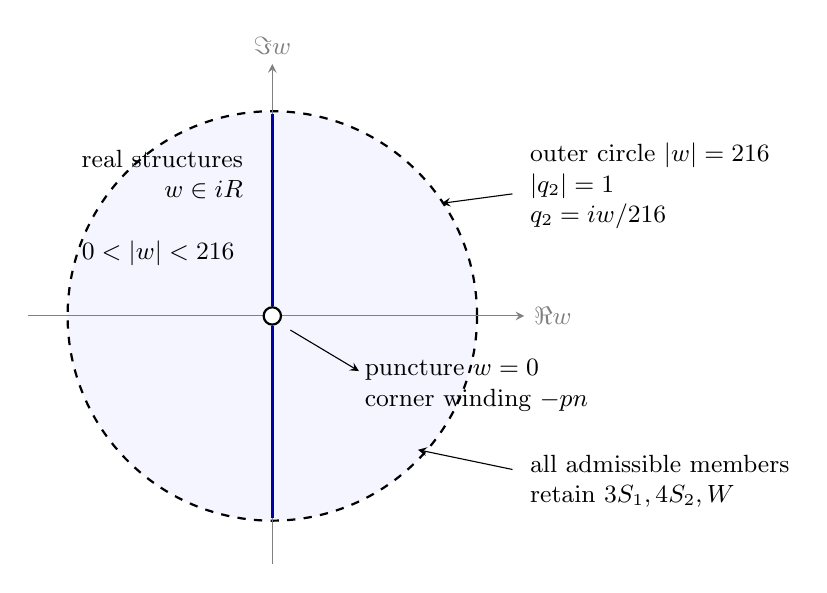
\begin{tikzpicture}[x=1cm,y=1cm,>=stealth,font=\small]
\fill[blue!4] (0,0) circle (2.6);
\draw[thick,dashed] (0,0) circle (2.6);
\draw[->,gray] (-3.1,0)--(3.2,0) node[right] {$\Re w$};
\draw[->,gray] (0,-3.15)--(0,3.2) node[above] {$\Im w$};
\draw[very thick,blue!65!black] (0,-2.56)--(0,-.13);
\draw[very thick,blue!65!black] (0,.13)--(0,2.56);
\fill[white] (0,0) circle (.11);
\draw[thick] (0,0) circle (.11);
\draw[->] (.23,-.18)--(1.1,-.7);
\node[anchor=west,align=left] at (1.05,-.88) {puncture $w=0$\\corner winding $-pn$};
\node[align=center] at (-1.45,.8) {$0<|w|<216$};
\node[anchor=west,align=left] at (3.15,1.65)
 {outer circle $|w|=216$\\$|q_2|=1$\\$q_2=iw/216$};
\draw[->] (3.05,1.55)--(2.15,1.43);
\node[anchor=east,align=right] at (-.25,1.8)
 {real structures\\$w\in i\mathbb R$};
\node[anchor=west,align=left] at (3.15,-2.1)
 {all admissible members\\retain $3S_1,4S_2,W$};
\draw[->] (3.05,-1.95)--(1.85,-1.7);
\end{tikzpicture}
\caption{The exact parameter disc for the standard fixed data.
The coordinate map is $w=e^{-\pi i c}$ and the coarser coordinate
map is $u=w^2$. The imaginary diameter is the fixed locus of
$w\mapsto-\bar w$, which is the reflected-family map.
The two boundary obstructions use the meridian comparison at the
puncture and the intrinsic Albanese nome at the outer circle.
The special fibres are over $t=0,1,\infty$ in every member, as
indicated in Figure~\ref{fig:I:orbifold}.}
\label{fig:I:parameter-disc}
\end{figure}

\begin{figure}[htbp]
\centering
\begin{tikzpicture}[x=1cm,y=1cm,>=stealth,font=\small]
\begin{scope}[shift={(-3.3,0)}]
 \fill[blue!5] (-1,0)--(-1,2.8)--(1,2.8)--(1,0)
  arc[start angle=30,end angle=150,radius=1.1547];
 \draw[thick] (-1,0)--(-1,2.8);
 \draw[thick] (1,0)--(1,2.8);
 \draw[thick] (1,0) arc[start angle=30,end angle=150,radius=1.1547];
 \node at (0,1.3) {$\mathcal F$};
 \node[align=center] at (0,-1.05)
 {$|\Re\tau|\le\tfrac12,\ |\tau|\ge1$\\$0\le\theta<\pi$};
 \draw[->] (0,2.1)--(0,3.1) node[above] {cusp};
\end{scope}
\begin{scope}[shift={(1.0,.2)},x={(1.8cm,0cm)},y={(.75cm,.5cm)},z={(0cm,2.2cm)}]
 \fill[blue!4] (0,0,0)--(1,0,0)--(1,0,1)--(0,0,1)--cycle;
 \draw[thick] (0,0,0)--(1,0,0)--(1,1,0)--(1,1,1)--(0,1,1)--(0,0,1)--cycle;
 \draw[thick] (1,0,0)--(1,0,1)--(0,0,1);
 \draw[thick] (1,0,1)--(1,1,1);
 \draw[dashed] (0,0,0)--(0,1,0)--(1,1,0);
 \draw[dashed] (0,1,0)--(0,1,1);
 \node[below] at (.5,0,0) {$0\le x_1<1$};
 \node[right] at (1,.5,0) {$0\le x_2<1$};
 \node[left] at (0,0,.5) {$0\le t<12$};
\end{scope}
\node[align=center] at (1.95,-1.55)
 {$U:\ t\mapsto t-6-6x_2$\qquad
  $V:\ t\mapsto t-6+6x_1$\\
  $Z:\ t\mapsto t+12$};
\end{tikzpicture}
\caption{A fundamental set for the index-twelve monodromy kernel
in the real parabolic stabilizer of $d$.
The base is a modular fundamental set with its rotation coordinate;
the fibre is the indicated Heisenberg parallelepiped. The displayed
face maps include the central shears. The representative map and
the boundary identifications are proved in
\ref{I:monodromy-fundamental-set}; the index twelve occurs in the
central fibre coordinate.}
\label{fig:I:monodromy-domain}
\end{figure}

\begin{proposition}[The fundamental set of the monodromy kernel]
\label{I:monodromy-fundamental-set}
\StatementRecord{I:monodromy-fundamental-set}{proved}{No earlier separately identified check is recorded. Checked only in this writing. Pre-continuation writing events: GPT-6 Astra (OpenAI), ChatGPT Pro mode, effort Pro, S6\_10\_PAPERS, 18 November 2026: targeted proof check. Continuation metadata events: GPT-6 Astra (OpenAI), ChatGPT Pro mode, effort Pro, S6\_10\_PAPERS continuation, 19 November 2026: used and rechecked in this run; status-vocabulary reconciliation; metadata reconciliation only; no new mathematical check. \emph{Pre-continuation recorded proof scope.} checked only in this writing by GPT-6 Astra (OpenAI), ChatGPT Pro mode, effort Pro, 18 November 2026}{\cref{fam:src:F.1.1,fam:src:F.1.2}; the displayed parabolic group law}
In the real coordinates $g(B,x,t)$ of
\ref{fam:src:F.1.1}, a measurable fundamental set for
$\Gamma\backslash P_d(\mathbb R)$ consists of the matrices
\[
 g(B,x,t),\qquad
 B=n(\Re\tau)a(\Im\tau)k(\theta),\quad
 \tau\in\mathcal F,\quad 0\le\theta<\pi,
 \quad x_1,x_2\in[0,1),\quad t\in[0,12).
\]
Here
$n(u)=\left(\begin{smallmatrix}1&u\\0&1\end{smallmatrix}\right)$,
$a(v)=\operatorname{diag}(\sqrt v,1/\sqrt v)$,
and $k(\theta)$ is the rotation matrix. Paired modular edges
are assigned to one side, and their lower-dimensional
stabilizer identifications use the corresponding lifts in
$\Gamma$: for
$S=\left(\begin{smallmatrix}0&-1\\1&0\end{smallmatrix}\right)$
and $T=\left(\begin{smallmatrix}1&1\\0&1\end{smallmatrix}\right)$,
we use $\widetilde S=g(S,0,9)$,
$\widetilde T=g(T,0,1)$ and
$\widetilde{-I}=g(-I,0,6)$.
Their maps on the three coordinates are
$(B,x,t)\mapsto(AB,Ax,t+\alpha(A))$, with
$\alpha(S)=9$, $\alpha(T)=1$ and $\alpha(-I)=6$.
The Heisenberg face identifications are the
maps printed in Figure~\ref{fig:I:monodromy-domain}.
\end{proposition}
\begin{proof}
\begin{enumerate}[label=\arabic*.,leftmargin=*]
\item The projection $g(B,x,t)\mapsto B$ maps $\Gamma$
onto $\operatorname{SL}_2(\mathbb Z)$ by
\ref{fam:src:F.1.1}. For any $B\in\operatorname{SL}_2(\mathbb R)$,
the usual modular reduction gives an integral matrix $A$
with $AB=n(u)a(v)k(\theta)$ in the stated set. Choose an
actual lift $g(A,y,s)\in\Gamma$ and multiply on the left.
For the displayed edge generators, the character formula
$\chi(g(A,0,t))=t-\alpha(A)\pmod {12}$ proves that the
three specified lifts lie in $\Gamma$. Substitution in
the group law gives each displayed coordinate map.
This is the specified map from a general parabolic element
to one over the modular set.
\item Two choices of lift over the same $A$ differ by
$\Gamma\cap H$. The group calculation in
\ref{fam:src:F.1.1} identifies this kernel with
$\langle U,V,Z\rangle$, where
$U=g(I,(1,0),-6)$, $V=g(I,(0,1),-6)$ and
$Z=g(I,0,12)$.
\item The multiplication law sends $(x,t)$ under $U$
to $(x+(1,0),t-6-6x_2)$, and under $V$ to
$(x+(0,1),t-6+6x_1)$. Powers of these maps first put
$x_1$ and $x_2$ in $[0,1)$. A power of $Z$ then puts
$t$ in $[0,12)$. All three are actual left translations
in $\Gamma$, so they retain the original coset.
\item Within the interiors of these intervals equality
of two reduced representatives forces their kernel
element to have zero $x$-translation and then zero
central translation. Modular uniqueness gives the same
conclusion in the base interior. The usual edge and
elliptic identifications, lifted by the specified
surjection, account for the measure-zero boundary.
This proves the fundamental-set assertion and all
displayed Heisenberg identifications.
\end{enumerate}
\end{proof}
